\documentclass[14pt,a4paper]{extarticle}

\usepackage{fontspec}
\usepackage{polyglossia}
\setdefaultlanguage{russian}
\setotherlanguage{english}

\setmainfont{Tinos}
\setsansfont{Arimo}
\setmonofont{Cousine}[Scale=0.82]

\usepackage{geometry}
\geometry{a4paper, top=2cm, bottom=2cm, left=3cm, right=1.5cm}

\usepackage{amsmath}
\usepackage{amssymb}
\usepackage{graphicx}
\usepackage{float}
\usepackage{booktabs}
\usepackage{xcolor}
\usepackage{listings}
\usepackage{caption} 
\usepackage{tikz}
\usetikzlibrary{positioning}
\usepackage{enumitem}
\usepackage{hyperref}

\hypersetup{hidelinks, unicode}

\linespread{1.3}
\emergencystretch=1.5em
\setlength{\parindent}{1.25cm}

\captionsetup[figure]{name=Рисунок, labelsep=endash}
\captionsetup[table]{name=Таблица, labelsep=endash, singlelinecheck=false, justification=raggedright}
\renewcommand{\lstlistingname}{Листинг}

\newcommand{\Student}{А. А. Устинов}
\newcommand{\Group}{М8О-307БВ-24}
\newcommand{\Teacher}{В. Д. Бахарев}
\newcommand{\Year}{2026}

\definecolor{codegray}{gray}{0.45}
\definecolor{codegreen}{rgb}{0.0,0.45,0.2}
\definecolor{codeblue}{rgb}{0.1,0.2,0.65}

\lstdefinestyle{code}{
	basicstyle=\ttfamily\footnotesize,
	keywordstyle=\color{codeblue}\bfseries,
	commentstyle=\color{codegreen}\itshape,
	stringstyle=\color{codegray},
	numbers=left,
	numberstyle=\tiny\color{codegray},
	numbersep=8pt,
	breaklines=true,
	breakatwhitespace=false,
	showstringspaces=false,
	tabsize=4,
	extendedchars=true,
	inputencoding=utf8,
	frame=single,
	rulecolor=\color{codegray},
	framesep=4pt,
	captionpos=b,
	texcl=true,
	literate={\ }{{\ }}1
}
\lstset{style=code, language=C++}

\lstdefinelanguage{GLSL}[]{C++}{
	morekeywords={vec2,vec3,vec4,mat2,mat3,mat4,layout,location,uniform,in,out,
		push_constant,gl_Position,mix,version,set,binding,std430,readonly,buffer,
		uint,struct,normalize,dot,max,pow,clamp,sqrt,transpose,inverse,
		sampler2D,texture,sin,cos,const},
}

\newcommand{\screenshot}[2]{%
	\begin{figure}[H]
		\centering
		\IfFileExists{#1}{%
			\includegraphics[width=0.92\textwidth]{#1}%
		}{%
			\fbox{\parbox[c][45mm][c]{0.9\textwidth}{\centering\itshape
				Место для скриншота\\[2pt]\ttfamily\small #1}}%
		}
		\caption{#2}
	\end{figure}}


\begin{document}

\begin{titlepage}
	\centering

	МОСКОВСКИЙ АВИАЦИОННЫЙ ИНСТИТУТ\par
	(НАЦИОНАЛЬНЫЙ ИССЛЕДОВАТЕЛЬСКИЙ УНИВЕРСИТЕТ)\par

	\vspace{6mm}

	Институт №8 <<Компьютерные науки и прикладная математика>>\par
	Кафедра 806 <<Вычислительная математика и программирование>>\par

	\vspace{6cm}

	{\Large Лабораторная работа №3\par}
	\vspace{3mm}
	{\large по курсу <<Компьютерная графика>>\par}
	\vspace{8mm}
	{\Large\bfseries Текстурирование\par}
	\vspace{3mm}
	{\large Объект: правильный октаэдр\par}

	\vspace{4cm}

	\begin{flushright}
		\begin{minipage}{0.5\textwidth}
			Выполнил: \Student\par
			Группа: \Group\par
			\vspace{6mm}
			Преподаватель: \Teacher\par
		\end{minipage}
	\end{flushright}

	\vfill
	Москва, \Year\par
\end{titlepage}

\section{Условие}

Цель работы — загрузить изображения из файловой системы, создать из них
текстуры и с помощью текстурных координат вершин и сэмплеров наложить их на
рисуемые объекты.

Объект — правильный октаэдр из первой лабораторной работы с освещением по
модели Блинна-Фонга из второй. Программа работает в реальном времени с
использованием Vulkan, GLFW и ImGui. Альбедо поверхности берётся из текстуры
вместо сплошного цвета. Изображения хранятся в файлах PNG и декодируются
сторонней библиотекой stb\_image. У вершин помимо позиции и нормали есть
текстурные координаты, которые генерируются процедурно вместе с геометрией.

Выполнено базовое задание:

\begin{itemize}[nosep, leftmargin=*]
	\item текстура накладывается на объекты как альбедо, без дополнительных
	эффектов;
	\item свойства всех моделей хранятся в одном динамическом uniform-буфере,
	а сдвиг до свойств конкретной модели задаётся в команде привязки набора
	дескрипторов;
	\item вершинные и индексные буферы находятся в памяти видеокарты (VRAM) и
	заполняются командами копирования из staging-буфера;
\end{itemize}

\noindent и два дополнительных задания:

\begin{enumerate}[nosep, leftmargin=*]
	\item загружается шесть текстур, для каждой модели текстура выбирается из
	выпадающего списка; у каждой текстуры свой набор дескрипторов;
	\item для одного объекта реализовано нетривиальное сэмплирование,
	зависящее от времени: искажение текстурных координат, две выборки одной
	текстуры разными координатами и модуляция цвета. Включается и
	настраивается эффект через push-константы.
\end{enumerate}

Для наглядности сцена расширена: октаэдр стоит в комнате из пола и трёх стен,
рядом с ним находятся ещё два октаэдра меньшего размера, вращающиеся вокруг
вертикальной оси. Всего на сцене семь моделей и три сетки.

% ------------------------------------------------------------------
\section{Метод решения}

\subsection{Текстуры и их загрузка}

Текстура — это изображение в памяти видеокарты, из которого шейдер читает
цвет по текстурным координатам $(u, v) \in [0, 1]^2$: точка $(0, 0)$
соответствует левому верхнему углу изображения, $(1, 1)$ — правому нижнему.
Отдельный пиксель текстуры называется текселем.

В работе используются шесть бесшовных изображений $512 \times 512$:
кирпичная кладка, деревянные доски, мрамор, лава, контрольная сетка с
подписанными клетками и каменная плитка (рис.~\ref{fig:set}). Изображения
построены из процедурного шума и сохранены в PNG; программа о способе их
создания ничего не знает и просто читает файлы.

\begin{figure}[H]
	\centering
	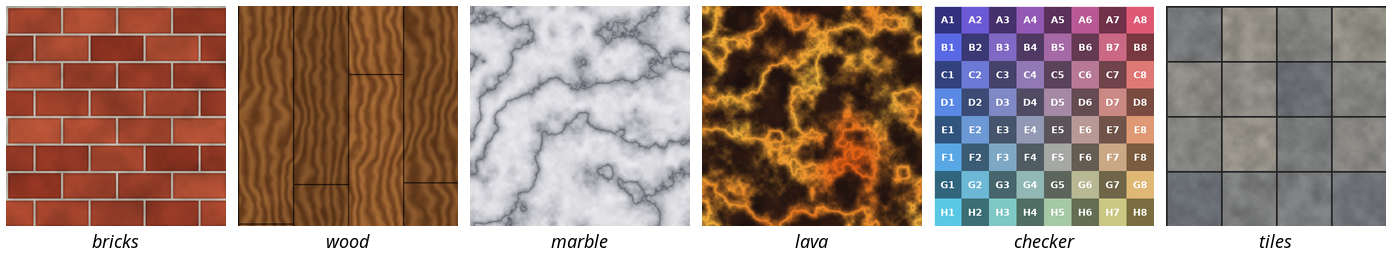
\includegraphics[width=\textwidth]{images/texture_set.png}
	\caption{Набор текстур}
	\label{fig:set}
\end{figure}

Файл декодирует функция \texttt{stbi\_load} библиотеки stb\_image. Она
поддерживает PNG, JPEG, BMP, TGA и другие форматы и всегда возвращает массив
пикселей по четыре байта (R, G, B, A), независимо от числа каналов в файле.

Дальше пиксели нужно переместить в изображение Vulkan. Изображение с
оптимальной для видеокарты раскладкой (\texttt{VK\_IMAGE\_TILING\_OPTIMAL})
располагается в VRAM, и записать в него напрямую процессор не может. Поэтому
пиксели сначала копируются в \textbf{staging-буфер} — промежуточный буфер в
памяти, доступной процессору, — а затем видеокарта сама переносит их в
изображение командой \texttt{vkCmdCopyBufferToImage}.

\textbf{Формат.} Изображение создаётся в формате
\texttt{VK\_FORMAT\_R8G8B8A8\_SRGB}. Цвета в PNG записаны в нелинейном
пространстве sRGB, а освещение должно считаться в линейном: складывать и
умножать имеет смысл физические величины, а не их гамма-кодированные
значения. Для формата \texttt{\_SRGB} видеокарта переводит тексели в
линейное пространство при чтении в шейдере, а кадр в формате sRGB при записи
кодирует обратно.

\textbf{Раскладки изображения.} Изображение Vulkan в каждый момент находится в
определённой раскладке (\texttt{VkImageLayout}), подходящей для конкретной
операции. Переходы выполняются барьерами \texttt{vkCmdPipelineBarrier}, которые
заодно гарантируют, что следующая операция начнётся только после завершения
предыдущей:

\begin{center}
	\begin{tabular}{@{}l l@{}}
		\toprule
		Раскладка & Для чего \\
		\midrule
		\texttt{UNDEFINED} & начальная, содержимое не определено \\
		\texttt{TRANSFER\_DST\_OPTIMAL} & приёмник копирования \\
		\texttt{TRANSFER\_SRC\_OPTIMAL} & источник копирования \\
		\texttt{SHADER\_READ\_ONLY\_OPTIMAL} & чтение из шейдера \\
		\bottomrule
	\end{tabular}
\end{center}

\textbf{Уровни детализации.} Если текстура на экране мельче, чем в файле
(например, дальняя часть пола), на один пиксель экрана приходится много
текселей. Выборка одного из них даёт мерцание и муар. Поэтому для каждой
текстуры строится цепочка уменьшенных копий (mip-уровней): каждый следующий
уровень вдвое меньше предыдущего, до размера $1 \times 1$. Их число

\begin{equation}
	L = \bigl\lfloor \log_2 \max(w, h) \bigr\rfloor + 1,
\end{equation}

для $512 \times 512$ это 10 уровней. Уровень $i$ получается из уровня $i - 1$
командой \texttt{vkCmdBlitImage} с линейной фильтрацией. Перед ней уровень
$i - 1$ переводится в раскладку источника, после — в раскладку для чтения
шейдером. Видеокарта сама выбирает нужный уровень по тому, насколько быстро
меняются текстурные координаты между соседними пикселями экрана. Если формат
не поддерживает такое копирование, программа обходится одним уровнем.

\textbf{Сэмплер} описывает, как читается текстура. В работе один сэмплер на
все текстуры: линейная фильтрация внутри уровня и между уровнями
(трилинейная) и режим адресации \texttt{REPEAT}, при котором координаты за
пределами $[0, 1]$ берутся по модулю, и текстура повторяется. Повторение
нужно полу и стенам, на которых текстура уложена несколько раз, и
анимированному эффекту, сдвигающему координаты.

\subsection{Текстурные координаты}

Текстурные координаты хранятся в каждой вершине вместе с позицией и нормалью
и генерируются процедурно.

\textbf{Пол и стены} — прямоугольники, заданные углом $\mathbf{o}$ и двумя
сторонами $\mathbf{e}_u$ и $\mathbf{e}_v$. Вершина с долями $(a, b)$ вдоль
сторон, $a, b \in \{0, 1\}$, получает

\begin{equation}
	\mathbf{p} = \mathbf{o} + a\,\mathbf{e}_u + b\,\mathbf{e}_v, \qquad
	(u, v) = \bigl(a\,n_u,\ (1 - b)\,n_v\bigr),
\end{equation}

где $n_u$ и $n_v$ — сколько раз текстура укладывается вдоль каждой стороны.
Координата $v$ отсчитывается от верхнего края, потому что строки изображения
идут сверху вниз; иначе кирпичи на стене оказались бы перевёрнутыми. Пол
$12 \times 12$ и стены шириной 12 получают по 4 повторения, стены высотой 4,5
— 1,5 повторения, так что одна плитка текстуры везде занимает квадрат
$3 \times 3$. Координаты больше единицы приводит к $[0, 1]$ режим
\texttt{REPEAT}.

\textbf{Октаэдр} развёрнут октаэдрической развёрткой, которая отображает
поверхность $|x| + |y| + |z| = 1$ на квадрат целиком. Верхняя половина
($y \ge 0$) проецируется на плоскость $XZ$, а нижняя <<раскрывается>> наружу:

\begin{equation}
	(u', v') =
	\begin{cases}
		(x,\ z), & y \ge 0, \\
		\bigl((1 - |z|)\operatorname{sgn} x,\ (1 - |x|)\operatorname{sgn} z\bigr), & y < 0,
	\end{cases}
	\label{eq:octa}
\end{equation}

\noindent после чего координаты переводятся из $[-1, 1]$ в $[0, 1]$:

\begin{equation}
	(u, v) = \left(\frac{u' + 1}{2},\ \frac{v' + 1}{2}\right).
\end{equation}

Четыре верхние грани занимают ромб в центре квадрата, нижние — четыре его
угла (рис.~\ref{fig:octa}). Это похоже на конверт: углы квадрата
загибаются к центру, и квадрат превращается в октаэдр. Каждая грань
отображается на треугольник площадью $1/8$ квадрата аффинно, без искажений,
поэтому плотность текселей на всех гранях одинакова и используется вся
текстура.

\begin{figure}[H]
	\centering
	\begin{tikzpicture}[scale=1.7, yscale=-1, font=\small]
		\fill[gray!12] (0,0) rectangle (4,4);
		\fill[blue!12] (2,0) -- (4,2) -- (2,4) -- (0,2) -- cycle;
		\draw[thick] (0,0) rectangle (4,4);
		\draw[thick] (2,0) -- (4,2) -- (2,4) -- (0,2) -- cycle;
		\draw (0,2) -- (4,2);
		\draw (2,0) -- (2,4);
		\node at (2.75,2.75) {$+x{+}z$};
		\node at (1.25,2.75) {$-x{+}z$};
		\node at (2.75,1.25) {$+x{-}z$};
		\node at (1.25,1.25) {$-x{-}z$};
		\node at (3.55,3.55) {$+x{+}z$};
		\node at (0.45,3.55) {$-x{+}z$};
		\node at (3.55,0.45) {$+x{-}z$};
		\node at (0.45,0.45) {$-x{-}z$};
		\fill (2,2) circle (1.5pt) node[above right] {$+y$};
		\foreach \p in {(0,0),(4,0),(0,4),(4,4)} \fill \p circle (1.5pt);
		\node[above left] at (0,0) {$-y$};
		\node[above right] at (4,0) {$-y$};
		\node[below left] at (0,4) {$-y$};
		\node[below right] at (4,4) {$-y$};
		\node[right] at (4,2) {$+x$};
		\node[left] at (0,2) {$-x$};
		\node[below] at (2,4) {$+z$};
		\node[above] at (2,0) {$-z$};
		\draw[->] (-0.6,-0.5) -- (0.4,-0.5) node[right] {$u$};
		\draw[->] (-0.6,-0.5) -- (-0.6,0.5) node[below] {$v$};
	\end{tikzpicture}
	\caption{Октаэдрическая развёртка. В ромбе (голубой) — верхние грани, в
	углах (серые) — нижние; подписаны знаки $x$ и $z$ грани. Вершина $-y$
	попадает во все четыре угла квадрата}
	\label{fig:octa}
\end{figure}

На рёбрах, соединяющих верхнюю и нижнюю половины, развёртка непрерывна: обе
грани отображают ребро на одну и ту же сторону ромба. Шов есть только на
четырёх рёбрах, сходящихся в нижней вершине: они лежат на границе квадрата,
и соседние грани берут тексели с противоположных его краёв.

Вершины октаэдра по-прежнему дублируются для каждой грани. Причин теперь две:
у граней разные нормали (это было и во второй работе), а нижняя вершина
получает в каждой из четырёх граней свои текстурные координаты — разные
углы квадрата. Принадлежность грани верхней или нижней половине и знаки в
формуле~\eqref{eq:octa} определяются по нормали грани, а не по вершине:
у вершин на <<экваторе>> $y = 0$, и по ним одним половину не определить. Для
таких вершин обе ветви формулы дают одинаковый результат, поэтому соседние
грани сходятся без разрыва.

\subsection{Вершины и индексы в VRAM}

Во второй работе вершинные буферы находились в памяти, доступной процессору:
видеокарта читала их через шину при каждом кадре. Теперь вершины и индексы
размещаются в VRAM, а копируются туда так же, как текстуры:

\begin{enumerate}[nosep, leftmargin=*]
	\item создаётся буфер в VRAM с назначением \texttt{VERTEX\_BUFFER} или
	\texttt{INDEX\_BUFFER} и \texttt{TRANSFER\_DST}; при выделении памяти
	библиотеке VMA передаётся \texttt{VMA\_MEMORY\_USAGE\_\allowbreak AUTO\_PREFER\_DEVICE}
	без флагов доступа процессора;
	\item данные копируются в staging-буфер в памяти процессора;
	\item в буфер команд записывается \texttt{vkCmdCopyBuffer} из
	staging-буфера в буфер VRAM.
\end{enumerate}

Все копирования при запуске — три сетки и шесть текстур — записываются в один
буфер команд и отправляются в очередь одним пакетом. В конце записывается
барьер, после которого результаты копирования видны этапу чтения вершин и
индексов. Программа дожидается выполнения (\texttt{vkQueueWaitIdle}), после
чего staging-буферы и пул команд уничтожаются.

Индексный буфер позволяет не хранить одинаковые вершины дважды. При
построении сетки вершина с теми же позицией, нормалью и текстурными
координатами, что уже есть в сетке, не добавляется, а в индексы записывается
номер существующей. У прямоугольника два треугольника дают 6 индексов на 4
вершины. У октаэдра повторов нет: 24 индекса на 24 вершины, поскольку у
каждой грани свои нормаль и координаты. Рисование выполняется командой
\texttt{vkCmdDrawIndexed} с 16-битными индексами.

\subsection{Динамический uniform-буфер}

Во второй работе у каждой модели был собственный uniform-буфер и собственный
набор дескрипторов. Теперь свойства всех моделей — матрица преобразования и
параметры блика — лежат в одном буфере массивом, а нужный элемент выбирается
при привязке набора.

Дескриптор типа \texttt{UNIFORM\_BUFFER\_DYNAMIC} хранит буфер и размер
одного элемента, а начальный сдвиг передаётся отдельно в каждой команде
\texttt{vkCmdBindDescriptorSets}. Шейдер видит одну структуру и не знает, что
она — часть массива.

Сдвиг обязан быть кратным пределу видеокарты $a$ — минимальному
выравниванию сдвига uniform-буфера
(\texttt{minUniform\-Buffer\-Offset\-Alignment}). Структура \texttt{ModelData}
занимает 80 байт (матрица $4 \times 4$ и вектор из четырёх чисел), поэтому шаг
между элементами округляется вверх, и модель с номером $i$ находится по сдвигу

\begin{equation}
	s = \left\lceil \frac{80}{a} \right\rceil a, \qquad
	\mathit{offset}_i = i \cdot s.
\end{equation}

На программном рендерере llvmpipe $a = 16$, и шаг равен 80 байтам; на
типичных дискретных видеокартах $a = 64$, и шаг — 128 байт. Каждый кадр
процессор записывает свойства всех моделей по своим сдвигам и один раз
сбрасывает кеш всего буфера.

Альбедо из свойств модели убрано: цвет поверхности теперь задаёт текстура. В
структуре остались матрица, цвет блика и коэффициент блеска.

\subsection{Наборы дескрипторов}

Внешние данные шейдеров разделены на два набора.

\textbf{Набор 0 — данные сцены}, без изменений со второй работы:
uniform-буфер с матрицей $P \cdot V$, положением камеры, рассеянным светом и
направленным источником (привязка 0) и storage-буферы с массивами точечных
источников и прожекторов (привязки 1 и 2).

\textbf{Набор 1 — модель и материал}:

\begin{itemize}[leftmargin=*, nosep]
	\item привязка 0 — динамический uniform-буфер со свойствами моделей;
	\item привязка 1 — кортеж изображение-сэмплер
	(\texttt{COMBINED\_IMAGE\_SAMPLER}) с текстурой альбедо.
\end{itemize}

В базовом задании все модели используют один такой набор: одна текстура и
один буфер, а модели различаются только сдвигом. В дополнительном
задании~1 таких наборов шесть, по одному на текстуру. Все они ссылаются на
один и тот же динамический буфер, а различаются изображением. Чтобы сменить
текстуру модели, достаточно привязать при её отрисовке другой набор:
пересоздавать или обновлять дескрипторы не нужно, поэтому текстура меняется
в интерфейсе мгновенно.

Порядок команд при отрисовке кадра:

\begin{enumerate}[nosep, leftmargin=*]
	\item привязать конвейер и набор сцены (один раз за кадр);
	\item для каждой модели $i$:
	\begin{itemize}[nosep]
		\item привязать набор её текстуры с динамическим сдвигом
		$\mathit{offset}_i$;
		\item записать push-константы эффекта;
		\item привязать вершинный и индексный буферы её сетки и нарисовать.
	\end{itemize}
\end{enumerate}

Три октаэдра используют одну сетку, а стены — другую: модели различаются
только матрицей в динамическом буфере. Сетка хранится в VRAM один раз.

\subsection{Нетривиальное сэмплирование}

Для дополнительного задания~2 во фрагментном шейдере реализован эффект
<<текущей>> поверхности. Обозначим $T(\mathbf{x})$ — выборку из текстуры
модели по координатам $\mathbf{x}$, $\mathbf{x}_0 = (u, v)$ — текстурные
координаты пикселя, $t$ — время, умноженное на скорость эффекта, $d$ — сила
искажения.

\textbf{1. Искажение координат.} К координатам прибавляются две бегущие
синусоидальные волны:

\begin{equation}
	\mathbf{w} = d \cdot \bigl(\sin(6\pi v + 2t),\ \ \sin(6\pi u + 1{,}6\,t)\bigr).
\end{equation}

Смещение по $u$ зависит от $v$, и наоборот, поэтому прямые линии текстуры
изгибаются волнами, а со временем волны бегут по поверхности.

\textbf{2. Две выборки одной текстуры разными координатами.} Первый слой
читается по искажённым координатам, равномерно сдвигающимся по диагонали;
второй — по координатам, увеличенным вдвое, искажённым в противоположную
сторону и медленно вращающимся вокруг центра развёртки
$\mathbf{c} = (0{,}5;\ 0{,}5)$:

\begin{equation}
	\mathbf{a} = T\bigl(\mathbf{x}_0 + \mathbf{w} + (0{,}05;\ 0{,}03)\,t\bigr),
	\qquad
	\mathbf{b} = T\bigl(2\,R(0{,}2\,t)(\mathbf{x}_0 - \mathbf{c}) + \mathbf{c} - \mathbf{w}\bigr),
\end{equation}

где $R(\alpha)$ — матрица поворота на угол $\alpha$. Слои объединяются
покомпонентным максимумом $\max(\mathbf{a}, \mathbf{b})$: светлые участки
обоих слоёв остаются видны, и рисунки двигаются друг сквозь друга. Режим
\texttt{REPEAT} делает сдвиг и увеличение координат бесшовными.

\textbf{3. Модуляция цвета.} Результат умножается на оттенок, плавно
обходящий цветовой круг, и на яркость, пульсирующую волной вдоль диагонали
развёртки:

\begin{gather}
	\mathbf{k}_d = 1{,}4\,\max(\mathbf{a}, \mathbf{b}) \odot \boldsymbol{\tau}\cdot \rho, \\
	\boldsymbol{\tau} = 0{,}6 + 0{,}4\cos\bigl(2\pi(0{,}08\,t + (0;\ 0{,}33;\ 0{,}67))\bigr), \\
	\rho = 0{,}85 + 0{,}15\sin\bigl(3t - 8(u + v)\bigr).
\end{gather}

Сдвиг фаз каналов на треть периода даёт поочерёдное усиление красного,
зелёного и синего, то есть поворот оттенка. Полученное $\mathbf{k}_d$ дальше
используется в модели Блинна-Фонга как обычное альбедо, поэтому объект с
эффектом освещается так же, как остальные.

\textbf{Push-константы.} Включение эффекта и его параметры передаются не в
uniform-буфере моделей, а в push-константах — небольшом блоке данных (по
стандарту гарантировано не меньше 128 байт), который записывается прямо в
буфер команд командой \texttt{vkCmdPushConstants}:

\begin{lstlisting}[language=GLSL, numbers=none]
layout(push_constant) uniform Effect {
	uint enabled;      // 0 - обычная выборка, 1 - анимированная
	float time;        // время в секундах
	float speed;       // множитель скорости
	float distortion;  // сила искажения
} effect;
\end{lstlisting}

Эти 16 байт записываются перед каждой отрисовкой, для моделей без эффекта
\texttt{enabled = 0}. Для них не нужны ни буфер, ни дескриптор, ни
выравнивание, а структура свойств модели не раздувается полями, нужными
одному объекту. Диапазон push-констант объявлен в раскладке конвейера только
для фрагментного шейдера.

\subsection{Используемые объекты Vulkan}

\begin{itemize}[leftmargin=*]
	\item \texttt{VkImage} и \texttt{VkImageView} — по одному на текстуру:
	изображение в VRAM со всеми mip-уровнями и вид на него для шейдера;

	\item \texttt{VkSampler} — один сэмплер на все текстуры;

	\item \texttt{VkBuffer} в VRAM — вершинный и индексный буферы каждой из
	трёх сеток (октаэдр, пол, стена);

	\item \texttt{VkBuffer} в памяти процессора — uniform-буфер сцены,
	storage-буферы источников, динамический uniform-буфер моделей и временные
	staging-буферы;

	\item \texttt{VkCommandPool} и \texttt{VkCommandBuffer} — для копирования
	данных в VRAM при запуске; уничтожаются сразу после копирования;

	\item \texttt{VkDescriptorSetLayout} — две раскладки: сцены и материала;

	\item \texttt{VkDescriptorPool} и \texttt{VkDescriptorSet} — один набор
	сцены и шесть наборов материалов. Все они заполняются один раз при
	запуске, поскольку ни буферы, ни изображения не пересоздаются;

	\item \texttt{VkPipelineLayout} — два набора дескрипторов и диапазон
	push-констант размером 16 байт;

	\item \texttt{VkPipeline} — графический конвейер. В формат вершины
	добавлен третий атрибут — текстурные координаты
	(\texttt{R32G32\_SFLOAT}); остальные настройки совпадают со второй
	работой.
\end{itemize}

\subsection{Интерфейс}

Раздел камеры и разделы источников света сохранены со второй работы. В новом
разделе моделей у каждой из семи моделей есть выпадающий список текстур
(дополнительное задание~1), положение, цвет блика и коэффициент блеска, у
октаэдров — масштаб и скорость вращения. Флажок <<Animated sampling>>
включает анимированное сэмплирование, а ползунки под ним задают скорость
эффекта и силу искажения (дополнительное задание~2). По умолчанию эффект
включён только у центрального октаэдра.

Ниже приведён фрагментный шейдер с выборкой из текстуры и анимированным
эффектом.

\lstinputlisting[language=GLSL, caption={Фрагментный шейдер: выборка из
текстуры, анимированное сэмплирование и модель Блинна-Фонга}]{shaders/textured.frag}

% ------------------------------------------------------------------
\section{Результаты}

\screenshot{images/scene.png}{Сцена при запуске. Пол — деревянные доски,
стены — кирпич, текстура на них повторяется. Центральный октаэдр — лава с
анимированным сэмплированием, слева — контрольная сетка, справа — мрамор}

\screenshot{images/uv.png}{Октаэдрическая развёртка на контрольной сетке.
Слева — вид сверху: верхние грани показывают центральный ромб текстуры
(в верхней вершине сходятся клетки D4, D5, E4 и E5, спереди видны строки
E--H). Справа — вид снизу: нижние грани показывают углы квадрата; надписи на
них повёрнуты, но не отражены зеркально, потому что развёртка сохраняет
ориентацию граней}

\screenshot{images/effect_checker.png}{Анимированное сэмплирование на
контрольной сетке. Слева сверху — эффект выключен, остальные кадры сняты с
интервалом около 1,5~с при включённом эффекте: видны два слоя текстуры
разного масштаба, волновое искажение надписей и смена оттенка}

\screenshot{images/effect_lava.png}{Тот же эффект на текстуре лавы. Слева
сверху — без эффекта; на остальных кадрах трещины двух слоёв перемещаются
друг относительно друга, а цвет переходит от красного к жёлто-зелёному}

\screenshot{images/textures.png}{Смена текстур через интерфейс: пол — каменная
плитка, задняя стена — доски, боковые — мрамор; центральный октаэдр — мрамор
без эффекта, правый — кирпич. Голубое пятно на полу — прожектор}

% ------------------------------------------------------------------
\section{Выводы}

В ходе работы я научился загружать изображения из файлов, создавать из них
текстуры Vulkan и накладывать их на объекты с помощью текстурных координат
и сэмплера, а также переносить данные в память видеокарты через
staging-буферы.

Главное, что я понял: копирование в VRAM — это не вызов
\texttt{memcpy}, а команда, которую выполняет видеокарта. Её нужно записать
в буфер команд, отправить в очередь и дождаться, а для изображений ещё и
явно перевести их из одной раскладки в другую барьерами. Зато после этого
вершины, индексы и текстуры лежат в быстрой памяти, и каждый кадр видеокарта
читает их, не обращаясь к памяти процессора.

Текстурные координаты, как и нормали во второй работе, оказались свойством
грани, а не вершины: нижняя вершина октаэдра получает в четырёх гранях
четыре разные пары координат. Октаэдрическая развёртка позволила уложить на
октаэдр всю текстуру целиком и без искажений, потому что каждая грань
отображается на свой треугольник квадрата аффинно.

Динамический uniform-буфер заменил множество отдельных буферов одним:
модели различаются только сдвигом при привязке набора. Наборы дескрипторов
на каждую текстуру позволяют сменить текстуру модели одной привязкой другого
набора, без обновления дескрипторов. Push-константы удобны для небольших
параметров, которые меняются от объекта к объекту, — флага и параметров
эффекта: они не требуют ни буфера, ни дескриптора.

\end{document}
